\section{test}
\label{sec:test}


\subsection{Datengrundlage und Datenakquisition}
Anknüpfend an die straßenbasierte Analyse nach Kaub et al. wird die OSM-Datengrundlage um funktionale Infrastrukturkomponenten erweitert \cite{kaub2024}.
Für die Modellierung des Strom- und Wassernetzes werden die \texttt{power} und \texttt{water} related Tags verwended \cite{osmwiki_features2026}.
Die ausreichende Datendichte für das Untersuchungsgebiet Trier wird exemplarisch in Abbildung~\ref{fig:infrastructure_data} über \textit{Open Infrastructure Map} nachgewiesen.

\begin{figure}[htbp]
    \centering
    \begin{subfigure}[b]{0.48\textwidth}
        \centering
        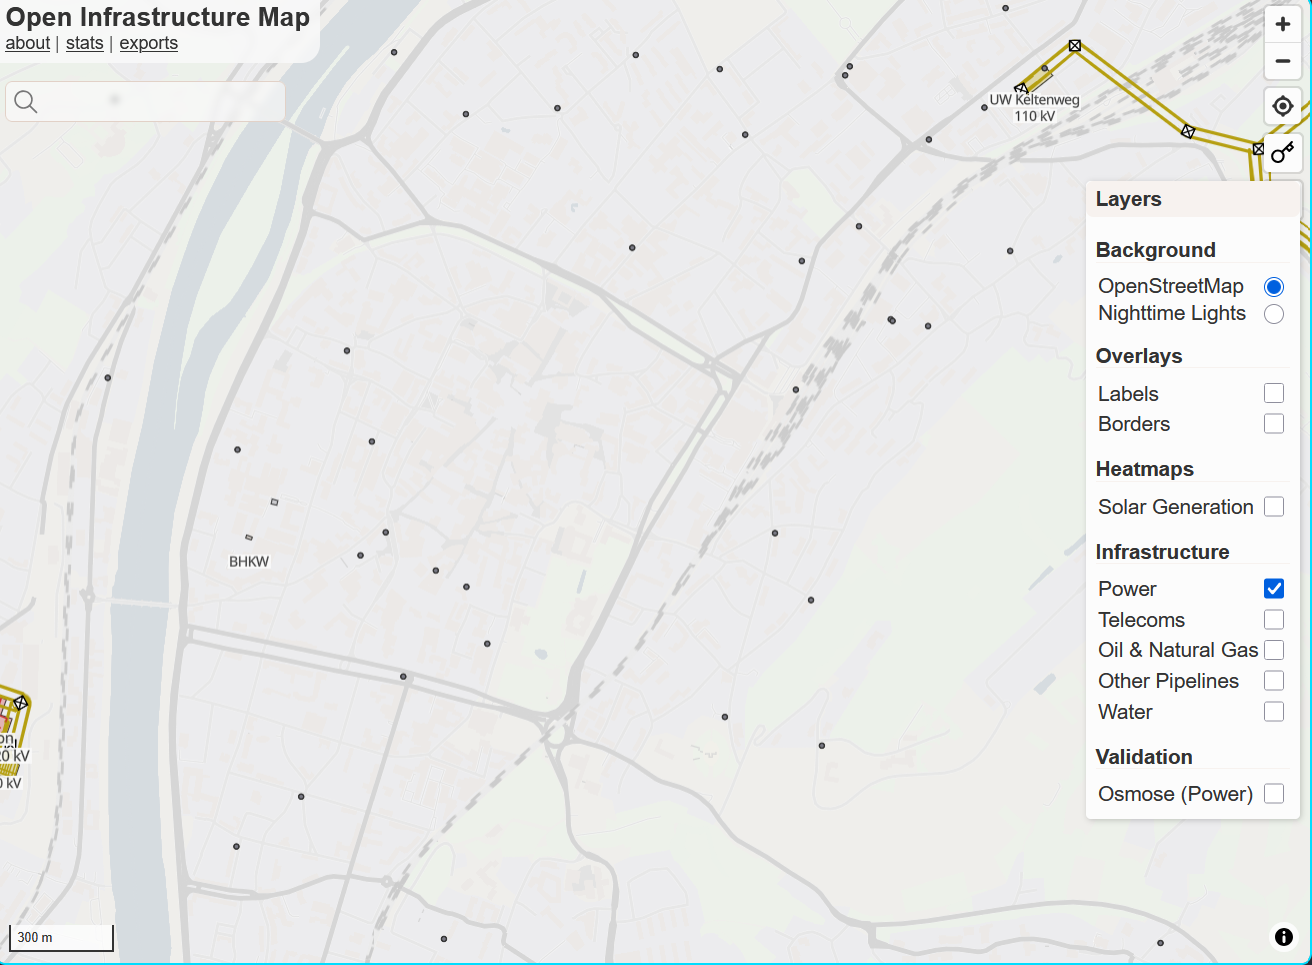
\includegraphics[width=\textwidth]{./resources/img_1}
        \caption{Verteilungsnetz und Substations}
        \label{fig:power_data}
    \end{subfigure}
    \hfill
    \begin{subfigure}[b]{0.48\textwidth}
        \centering
        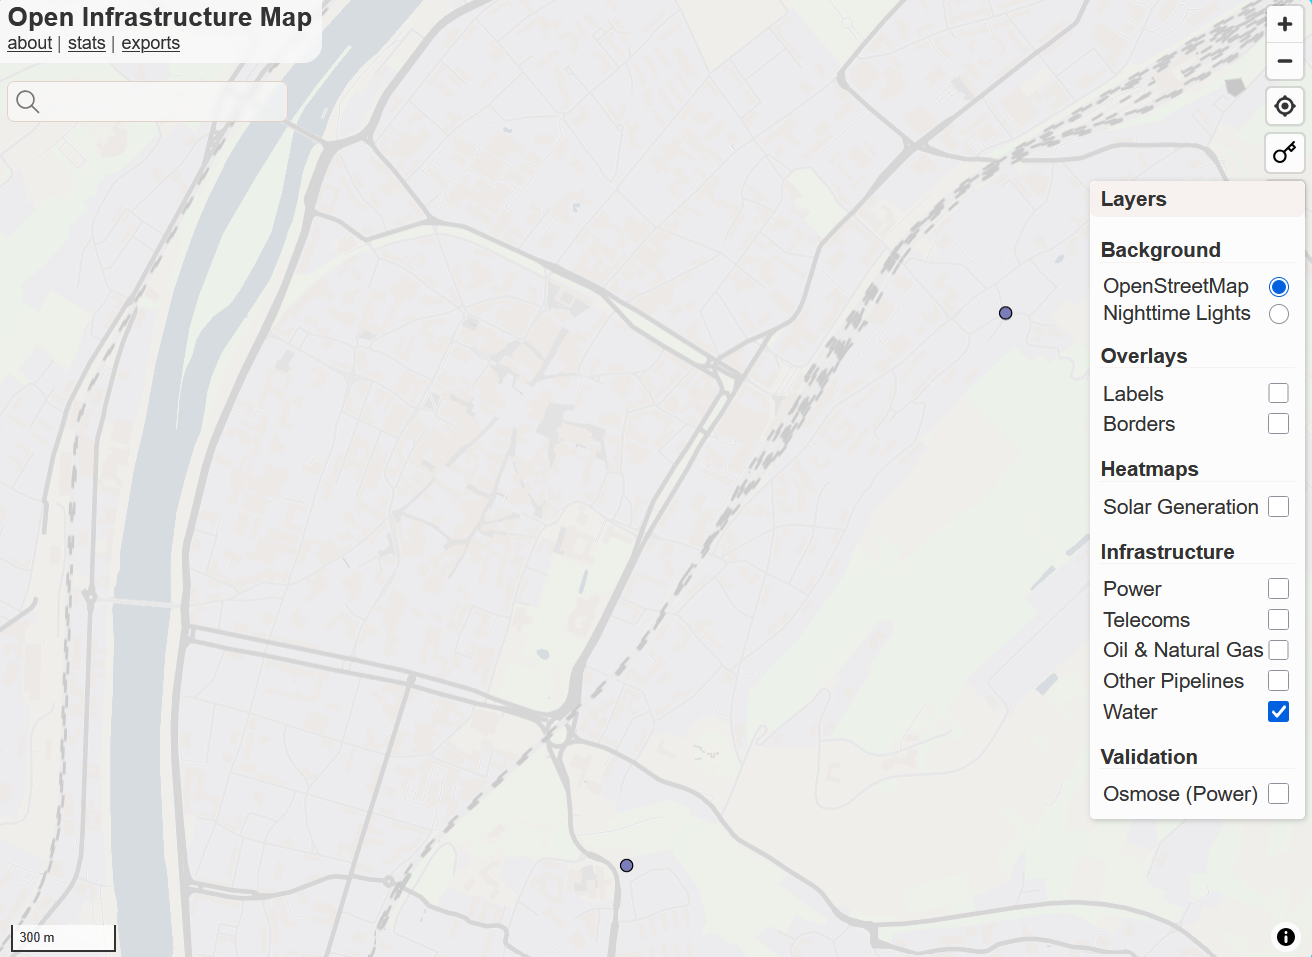
\includegraphics[width=\textwidth]{./resources/img}
        \caption{Wasserquellen und Fontänen}
        \label{fig:water_data}
    \end{subfigure}
    \caption{Visualisierung der zugrundeliegenden Infrastrukturdaten in Trier via Open Infrastructure Map.}
    \label{fig:infrastructure_data}
\end{figure}

\subsection{Topologische Kopplung und Netzwerkkartierung (The ``How'')}
Die Zuordnung zwischen POIs und Versorgungsnetzknoten erfolgt in der Literatur, etwa bei Lickert et al., über eine reine Luftlinien-Näherung (\textit{Euclidean Nearest-Neighbor} implementiert durch K-Nearest Neighbor (KNN)), was jedoch urbane topologische Barrieren vernachlässigt \cite{lickert2024}. Diese Arbeit implementiert daher den von Okabe et. al. geprägten \textit{Network-constrained Nearest-Neighbor} (NCNN) Ansatz \cite{okabe2012}. Dies erlaubt eine wesentlich realitätsnähere und zugleich simulationsbedingt effiziente Abbildung, da die Versorgungswege analog zum realen Straßennetz modelliert werden.

Sei $G = (V, E)$ der ungestörte Straßengraph \cite{cite: 88}. Für jeden kritischen Infrastrukturknoten $j$ wird das minimale Routing-Investment zu allen verfügbaren Strom- und Wasserverteilern berechnet \cite{cite: 96}:
\begin{equation}
    c(s_j, d_{\text{Infr}}) = \min_{d \in D_{\text{Infr}}} \text{Dijkstra}(s_j, d)
\end{equation}
Die so identifizierten Versorgungsbeziehungen werden zu Beginn der Simulation ($t_0$) fixiert und bilden das statische logische Netz der funktionalen Abhängigkeiten.

\subsection{Simulationsdesign und Multi-Tier-Validierung}
Die straßenbasierte Kopplung erhöht den geografischen Realismus und ermöglicht eine dreistufige Evaluierung der Systemresilienz. Zur Isolation der Modellkomplexität und Validierung des Frameworks werden drei Szenariostufen definiert:

\begin{enumerate}
    \item \textbf{Level A (Regression Control):} Schränkt die Simulation auf physische Straßenblockaden bei permanent intakten Versorgungsnetzen ein ($x_{\text{Strom}}(t) = 1, x_{\text{Wasser}}(t) = 1$). Als Regressionstest müssen die Ergebnisse exakt dem ursprünglichen RoA-Index entsprechen, um die Integrität der erweiterten Routing-Logik zu validieren.

    \item \textbf{Level B (Power Cascade):} Schaltet das Stromnetz frei. Überflutete Umspannwerke fallen zum Zeitpunkt $t_{\text{off}}$ aus. Nach Ablauf des Puffers ($\Delta t_{\text{puffer}}$) verliert der zugeordnete POI seine funktionale Betriebsfähigkeit ($x_{\text{Strom}}(t) = 0$), was trotz physischer Erreichbarkeit den ``funktionalen Gap'' isoliert.

    \item \textbf{Level C (Compound Failure):} Bildet die höchste Komplexitätsstufe ab, in der alle Kanäle simultan bedient werden müssen ($\forall i \in I: x_i(t) > 0$). Fällt mindestens ein Kanal (Straße, Strom oder Wasser) aus, bricht die funktionale Gesamtverfügbarkeit ein ($\Phi_j(t) = 0$).
\end{enumerate}

\noindent
Dieses gestaffelte Design identifiziert kritische Kipppunkte und prüft die zentrale Hypothese, dass rein straßenbasierte Modelle die urbane Krisenresilienz signifikant überschätzen. Die unstehende Grafik veranschalicht den Funktionalen Gap sowie das vorgehen wo Wasser, Strom und Straße über die gleichen Kanten verlaufen

\begin{figure}[htbp]
    \centering
    \begin{subfigure}[b]{0.32\textwidth}
        \centering
        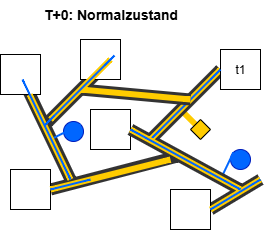
\includegraphics[width=\textwidth]{./resources/normal}
        \caption{$T+0$: Normalzustand des Systems}
        \label{fig:t0_normal}
    \end{subfigure}
    \hfill
    \begin{subfigure}[b]{0.32\textwidth}
        \centering
        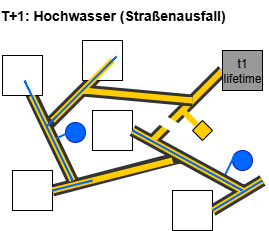
\includegraphics[width=\textwidth]{./resources/ausfall.png}
        \caption{$T+1$: Straßenausfall (Puffer)}
        \label{fig:t1_ausfall}
    \end{subfigure}
    \hfill
    \begin{subfigure}[b]{0.32\textwidth}
        \centering
        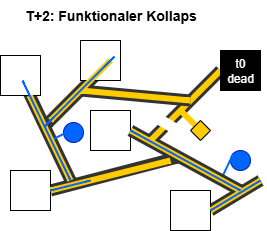
\includegraphics[width=\textwidth]{./resources/tot.png}
        \caption{$T+2$: Funktionaler Kollaps}
        \label{fig:t2_kollaps}
    \end{subfigure}
    \caption{Simulierte Kaskadenentwicklung: Vom ungestörten Zustand ($T+0$) über den physischen Infrastrukturausfall bei aktiver Pufferzeit ($T+1$) bis hin zum vollständigen funktionalen Kollaps des POIs ($T+2$).}
    \label{fig:cascade_timeline}
\end{figure}